\documentclass[tikz,border=0pt]{standalone}
\usepackage[american]{circuitikz}
\usetikzlibrary{arrows.meta,calc,positioning,decorations.pathmorphing,patterns}
\definecolor{zyloTeal}{HTML}{174A5B}
\definecolor{zyloTealTwo}{HTML}{246B7A}
\definecolor{zyloInk}{HTML}{1F2933}
\definecolor{zyloSoft}{HTML}{EAF4F4}
\definecolor{zyloPaper}{HTML}{F8FAFB}
\definecolor{zyloLine}{HTML}{44606B}
\definecolor{zyloOrange}{HTML}{D97706}
\begin{document}
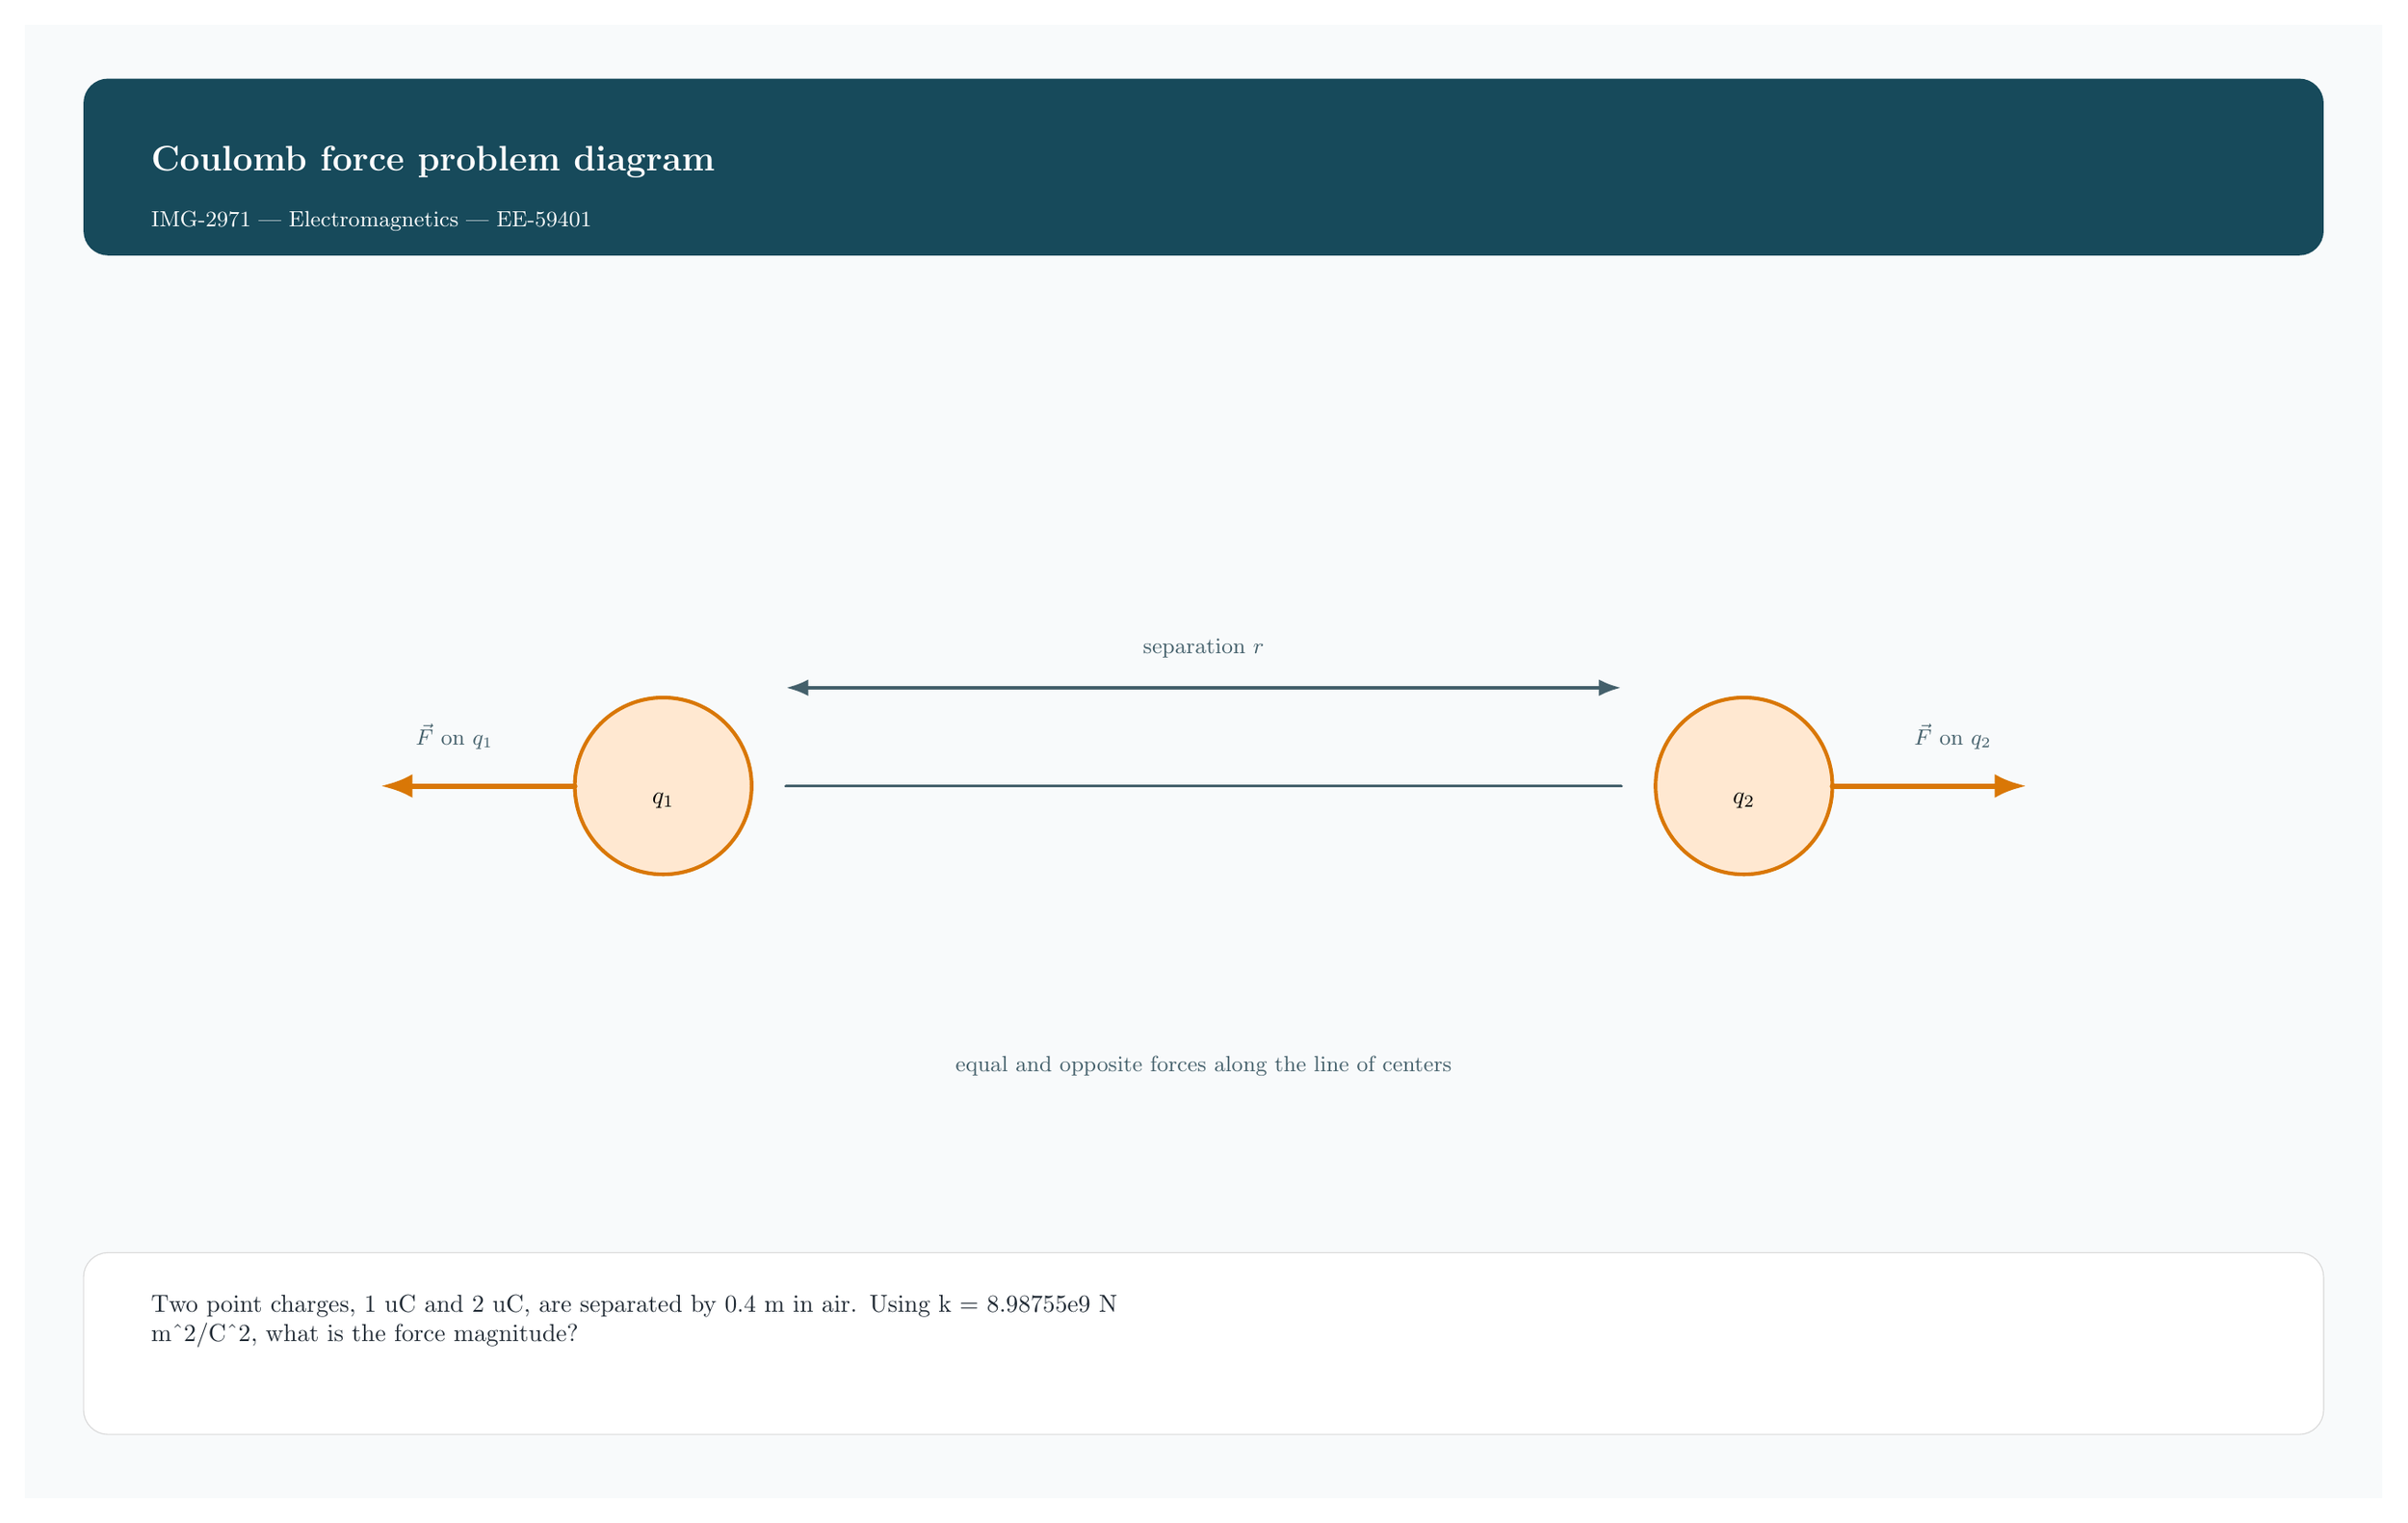
\begin{tikzpicture}[x=1pt,y=-1pt,>=Latex,line cap=round,line join=round]
\path[fill=zyloPaper] (0,0) rectangle (960,600);
\path[fill=zyloTeal,rounded corners=10pt] (24,22) rectangle (936,94);
\node[anchor=west,text=white,font=\bfseries\Large] at (48,56) {Coulomb force problem diagram};
\node[anchor=west,text=white!82,font=\small] at (48,80) {IMG-2971 | Electromagnetics | EE-59401};
\tikzset{wire/.style={draw=zyloTeal,line width=2.2pt},thinwire/.style={draw=zyloLine,line width=1.35pt},accent/.style={draw=zyloOrange,line width=2.2pt},box/.style={draw=zyloTealTwo,fill=zyloSoft,line width=1.5pt,rounded corners=8pt}}
\draw[draw=zyloOrange,fill=orange!18,line width=1.5pt] (260,310) circle (36); \draw[draw=zyloOrange,fill=orange!18,line width=1.5pt] (700,310) circle (36);
\node at (260,316) {$q_1$}; \node at (700,316) {$q_2$};
\draw[thinwire] (310,310) -- (650,310); \draw[thinwire,<->] (310,270) -- (650,270); \node[font=\small,text=zyloLine] at (480,254) {separation $r$};
\draw[accent,->] (224,310) -- (145,310); \draw[accent,->] (736,310) -- (815,310);
\node[font=\small,text=zyloLine] at (175,290) {$\vec F$ on $q_1$}; \node[font=\small,text=zyloLine] at (785,290) {$\vec F$ on $q_2$};
\node[font=\small,text=zyloLine] at (480,424) {equal and opposite forces along the line of centers};
\path[draw=black!15,fill=white,rounded corners=10pt] (24,500) rectangle (936,574);
\node[anchor=west,text width=860pt,align=left,text=zyloInk,font=\normalsize] at (48,528) {Two point charges, 1 uC and 2 uC, are separated by 0.4 m in air. Using k = 8.98755e9 N\\m\textasciicircum{}2/C\textasciicircum{}2, what is the force magnitude?};
\end{tikzpicture}
\end{document}
